\documentclass[12pt,fleqn]{article}\usepackage{../common}
\begin{document}
Kisitli Boltzmann Makinalari (Restricted Boltzmann Machines -RBM-)

Bir RBM icinde ikisel (binary) degerler tasiyan gizli (hidden) $h$
degiskenler, ve yine ikisel gorunen (visible) degiskenler $v$ vardir. $Z$
aynen once gordugumuz Boltzman Makinalarinda (BM) oldugu gibi normalizasyon
sabitidir.

$$ p(x,h;W) = \exp (-E(x,h)) / Z $$

$E$ tanimina ``enerji'' olarak atif yapildigini da gorebilirsiniz bazen. 

$$ E(x,h) = -h^TWx - c^Tx - b^Th $$

Dikkat edilirse, BM'lerden farkli olarak RBM taniminda $c,b$ degiskenleri
var. Bu degiskenler yanlilik (bias) icindir, yani veri icindeki genel
egilimi saptamalari icin modele konulmustur. Ayrica $h^TWx$ terimi var, bu
BM'deki $x^TWx$ biraz farkli, simdi gizli degiskenler, $h$ uzerinden
$x$'ler arasinda baglanti yapiyor. Bir baska ilginc farklilik BM ile tum
$x$' ogeleri birbirine baglanabiliyordu, RBM ile daha az (ya da fazla)
olabilecek $h$ katmaninda baglantilar paylasiliyor. Ozellikle azaltma
durumunda RBM ozellik alanini azaltarak bir tur genelleme eylemini
beceriyor.

Ustteki formul alttaki gibi acilabilir,

$$ = - \sum_j \sum_k W_{j,k}h_jx_k - \sum_k c_kx_k - \sum_j b_jh_j  $$

Dikkat: $h,x$ degiskenleri olasilik teorisinden bilinen rasgele
degiskenlerdir, yani hem $x$'e hem de $h$'e ``zar attirabiliriz'' / bu
degiskenler uzerinden orneklem toplayabiliriz. Bu kritik bir konu. Ayrica,
ustteki tanimlardan net sekilde anlasiliyor ama bir daha vurgulayalim;
RBM'ler aynen BM'ler gibi bir olasilik dagilimi uzerinden
tanimlanirlar. Tum mumkun degerleri uzerinden entegralleri (ya da
toplamlari) alininca sonuc 1 olur, vs.

RBM'lerin alttaki gibi resmedildigini gorebilirsiniz.

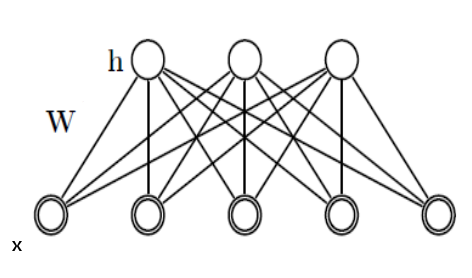
\includegraphics[height=4cm]{rbm_01.png}
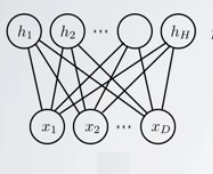
\includegraphics[height=4cm]{rbm_02.png}

RBM'lerin ``kisitli'' olarak tanimlanmalarinin sebebi, gizli degiskenlerin
kendi aralarinda, ve gorunen degiskenlerin kendi aralarinda direk
baglantiya izin verilmis olmasidir, bu bakimdan
``kisitlanmislardir''. Baglantilara, $W$ uzerinden sadece gizli ve gorunen
degiskenler (tabakalar) arasinda izin verilmistir. Bu tabii ki matematiksel
olarak bazi kolayliklar sagliyor.

Devam edelim, ana formulden hareketle cebirsel olarak sunlar da dogrudur,

$$ p(x,h;W) = \exp (-E(x,h)) / Z $$

$$ = \exp (h^TWx + c^Tx + b^Th ) / Z $$

$$ = \exp (h^TWx) \exp (c^Tx) \exp(b^Th) / Z $$

cunku bir toplam uzerindeki $\exp$, ayri ayri $\exp$'lerin carpimi
olur. Ayni mantikla, eger ana formulu matris / vektor yerine ayri
degiskenler olarak gormek istersek,

$$ 
p(x,h;W) = \frac{1}{Z}
\prod_j \prod_k \exp (W_{jk}h_jx_k) \prod_k \exp(c_kx_k) \prod_j \exp(b_jh_j) 
 $$

Notasyonu kolaylastirmak amaciyla $b,c$ terimlerini $W$ icine absorbe
edebiliriz, $x_0=1$ ve $h_0=1$ degerlerini mecbur tutarsak ve $w_{0,:}=c$
ve $w_{:,0}=b$ dersek, yani $W$'nin sifirinci satirinin tamamini $c$'ye set
edip, sifirinci kolonunun tamamini $b$'ye set edersek, RBM ana formulunu
tekrar elde etmis oluruz, fakat artik 

$$ E(x,h) = -h^TWx $$


$$ = - \sum_j \sum_k W_{j,k}h_jx_k  $$

ve
$$ p(x,h;W)  = \exp (h^TWx) / Z $$


Eger $y \equiv (x,h)$ olarak alirsak, 


$$ P(x,h;W) = \frac{1}{Z(W)} \exp 
\bigg[ 
\frac{1}{2} y^T W y
\bigg]
$$

$h$ uzerinden marjinalize edersek,

$$ P(x;W) = \sum_h \frac{1}{Z(W)} \exp 
\bigg[ 
\frac{1}{2} y^T W y
\bigg]
$$


$$  
\mlabel{1}
= \frac{1}{Z(W)}  \sum_h \exp 
\bigg[ 
\frac{1}{2} y^T W y
\bigg]
$$


And $Z(W)$ itself is
$$ Z(W) = \sum_{h,x} \exp 
\bigg[ 
\frac{1}{2} y^T W y
\bigg]
$$

(1) denkleminde bolumunden sonraki kisma $Z_x(W)$ dersek, sanki ayni $\exp$
denkleminin ``farkli bir sekilde marjinalize edilmis hali'' olarak
gostermis oluruz onu, ve boylece daha kisa bir formul kullanabiliriz,

$$  
= \frac{1}{Z(W)}  
\underbrace{
\sum_h \exp 
\bigg[ 
\frac{1}{2} y^T W y
\bigg]
}_{Z_x(W)}
$$
O zaman 

$$  
P(x;W) = \frac{Z_x(W)}{Z(W)}  
$$

elde ederiz. Veri uzerinden maksimum olurluk icin, yine log uzerinden bir
hesap yapariz, BM icin yapmistik bunu,

$$  
\mathcal{L} = 
\ln \big( \prod_{n=1}^{N} P(x^{n};W) \big) = 
\sum_{n=1}^{N} \ln P(x^{n};W) \big) 
$$

$$ 
=  \sum_{n=1}^{N} \ln \frac{Z_{x^{(n)}}(W)}{Z(W)}  
= \sum_{n=1}^{N}  \big(\ln Z_{x^{(n)}} - \ln Z \big)
 $$


$$ 
\frac{\partial \mathcal{L} }{\partial w_{ij}} = 
 \sum_{n=1}^{N}  \big( \frac{\partial \ln Z_{x^{(n)}} }{\partial w_{ij}}
- \frac{\partial \ln Z }{\partial w_{ij}} \big)
$$















\end{document}
